\documentclass{report}
\usepackage[margin=1in, paperwidth=8.5in, paperheight=11in]{geometry}
%Math packages%
\usepackage{amsmath}
\usepackage{amsthm}
%Spacing%
\usepackage{setspace}
%Package to adjust indentation%
\usepackage{changepage}
\onehalfspacing
%Lecture number%
\newcommand{\lectureNum}{12}
%Variables - Date and Course%
\newcommand{\curDate}{February 9, 2017}
\newcommand{\course}{CS 240}
%Defining the example tag%
%\theoremstyle{definition}%
\newtheorem{ex}{Example}[section]
%Setting counter given the lecture number%
\setcounter{chapter}{\lectureNum{}}
%Package to insert code%
\usepackage{listings}
\usepackage{courier}
\usepackage{xcolor}
\lstset { 
    tabsize=2,
    breaklines=true,
    language=C++,
    backgroundcolor=\color{blue!8}, % set backgroundcolor
    basicstyle=\footnotesize\ttfamily,% basic font setting
}
%Package to draw trees%
\usepackage{tikz}


\begin{document}
%Note title%
\begin{center}
\begin{Large}
\textsc{\course{} | Lecture \lectureNum{}}
\end{Large}
\end{center} 
\noindent \textit{Bartosz Antczak} \hfill
\textit{Instructor: Eric Schost} \hfill
\textit{\curDate{}}
\rule{\textwidth}{0.4pt}

% Actual Notes%
\subsubsection{Midterm Info}
Tries will be the last topic covered that will be on the midterm. Advice to do well on the midterm:
\begin{itemize}
\item Understand everything on the assignments. Practice them.
\item Understand all of the data structures we've gone through.
\end{itemize}
\section{Tries}
A \textbf{trie} (pronounced ``try", even though that's a ridiculous pronunciation personally) is a dictionary for binary strings, structured as a radix tree. A trie is structured such that:
\begin{itemize}
\item the left child corresponds to a 0 bit
\item the right child corresponds to a 1 bit
\end{itemize}
A node in the tree is \textit{flagged} if the path from the root to the node is a binary string that's present in the dictionary.
\begin{ex}
A trie for a particular set of binary strings (flagged nodes are in pink)
\end{ex}
\begin{figure}[ht]
\begin{center}
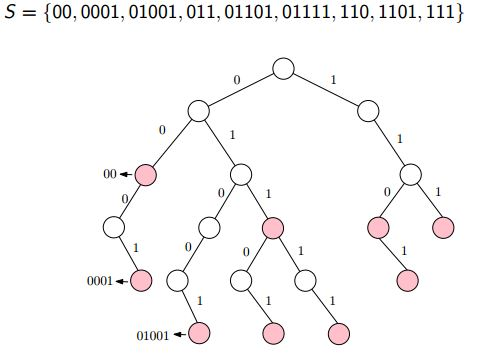
\includegraphics[scale=0.75]{trie1.jpg}
\end{center}
\caption{Courtesy of the CS 240 lecture slides.}
\end{figure}
\subsection{Search}
To find a particular string $x$ in the trie:
\begin{itemize}
\item Start at the root.
\item If the current bit in $x$ is 0, take the right link; otherwise, take the left link. Return failure if the link is missing.
\item If there are no extra bits in $x$ left and the current node is flagged, then return success (i.e., $x$ is found). If the node is not flagged, return failure.
\item Recurse.
\end{itemize}
\subsection{Insert}
To insert a binary string $x$ in the trie:
\begin{itemize}
\item Search for $x$, and suppose we finish at node $v$ (we finish at a node if the next bit value is not a child of the current node).
\item If $x$ still has extra bits, then expand the trie from node $v$ by adding necessary nodes that correspond to extra bits of $x$; flag the last one.
\end{itemize}
\subsection{Delete}
To delete a binary string $x$ in the trie:
\begin{itemize}
\item Search for $x$.
\item If $x$ is found at an internal flagged node (i.e., not a leaf), then unflag the node.
\item If $x$ is found at a leaf $v_x$, delete the leaf and all ancestors of $v_x$ until:
\begin{itemize}
\item We reach an ancestor that has two children, or
\item We reach a flagged node.
\end{itemize}
\end{itemize}
\subsection{Operation Time Complexity}
All three of these operations have a runtime of $\Theta(|x|)$, where $|x|$ is the length of the binary string (i.e., the number of bits in $x$).
\section{Compressed Tries}
Also called \textit{Patricia Tries}. Patricia stands for Practical Algorithm To Retrieve Information Coded In Alphanumeric (I wonder how long it took to think of that). This data structure reduces storage requirements by eliminating unflagged nodes with only one child.\\Each node stores a number representing the index value in the string that will be tested next (0 for the first bit, 1 for the second bit, etc.; just like an index for an array). A compressed trie storing $n$ keys always has at most $n-1$ internal (non-leaf) nodes. \newline
\begin{ex}
A trie with its respective compressed trie
\end{ex}
\begin{figure}[ht]
\begin{center}
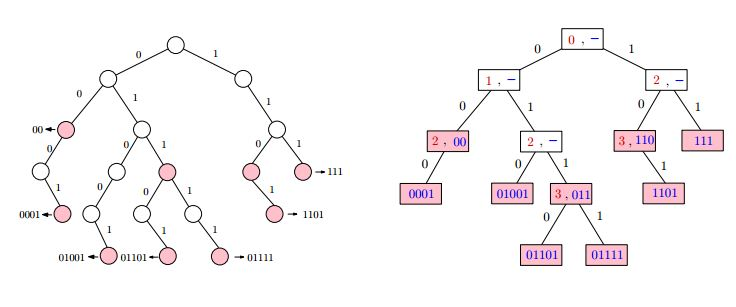
\includegraphics[scale=0.8]{trie2.jpg}
\end{center}
\caption{Courtesy of the CS 240 lecture slides.}
\end{figure}
\noindent Observe that the right child of the root has been reduced. The right child node contains an index number `2', which means that rather than checking the 1st index of the string,  skip directly to the second index and check what value it is.
\subsection{Claim 1}
\begin{center}
\textit{In a compressed trie with $n$ keys and $m$ internal nodes $m \leq n-1$}
\end{center}
\begin{adjustwidth}{0.5cm}{}
\subsubsection{Subclaim 1}
\begin{center}
\textit{In a complete (i.e., every node has 0 or 2 children) binary tree with n leaves, there are $n-1$ internal nodes}
\end{center}
The proof of this claim is done by induction and is left as an exercise.\\
\end{adjustwidth}
Define $n = n_1 + n_2 + n_3$ n1 are leaves, n2 have both children, n3 have one child.
Delete the n3 nodes (keys with one child), what is left is a complete binary tree with n1 leaves. It must jave n1 - 1 internal nodes.
We used to have m internal nodes but deleted n3 of those, so we have m-n3 internal nodes left. $$m-n_3 = n_1 - 1$$
So m = n1 + n3 - 1 $\leq n_1 + n_2 + n_3 - 1 = n - 1$.
\subsection{Search in a Compressed Trie}
To search for a binary string $x$ in a compressed trie:
\begin{itemize}
\item Follow the proper path from the root down in the tree to a leaf.
\item If the search ends in an unflagged node, it is unsuccessful.
\item If the search ends in a flagged node, we need to check if the key stored in indeed $x$.
\end{itemize}
\subsection{Delete}
To delete a string $x$ in a compressed trie:
\begin{itemize}
\item Perform \texttt{search(x)}.
\item If the search ends in an internal node:
\begin{itemize}
\item If the node has two children, then unflag the node and delete the key;
\item otherwise, delete the node and make their only child, the child of its parent
\end{itemize}
\item If the search ends in a leaf, then delete the leaf, and
\item if its parent is unflagged, then delete the parent.
\end{itemize}
\subsection{Insert}
This one's a doozy. To insert a string $x$ into a compressed trie:
\begin{itemize}
\item Perform \texttt{search(x)}.
\item If the search ends at a leaf $L$ with key $y$, compare $x$ against $y$.
\item If $y$ is a prefix of $x$, add a child to $y$ containing $x$.
\item Else, determine the first index $i$ where they disagree (i.e., they're not the same bit value) and create a new node $N$ with index $i$.\\
Insert $N$ along the path from the root to $L$ so that the parent of $N$ has index less than $i$ and one child of $N$ is either $L$ or an existing node on the path from the root to $L$ that has index greater than $i$.\\The other child of $N$ will be a new leaf node containing $x$.
\item If the search ends at an internal node, we find the key corresponding to that internal node and proceed in a similar way to the previous case.
\end{itemize}
\begin{ex}
Insert 1110 into an existing trie.
\end{ex}
\begin{itemize}
\item Search, arrive at 1100.
\item The first index where 1100 and 1110 differ is at index 2 $\rightarrow$ so create a new node to test index 2.
\end{itemize}
\begin{figure}[ht]
\begin{center}
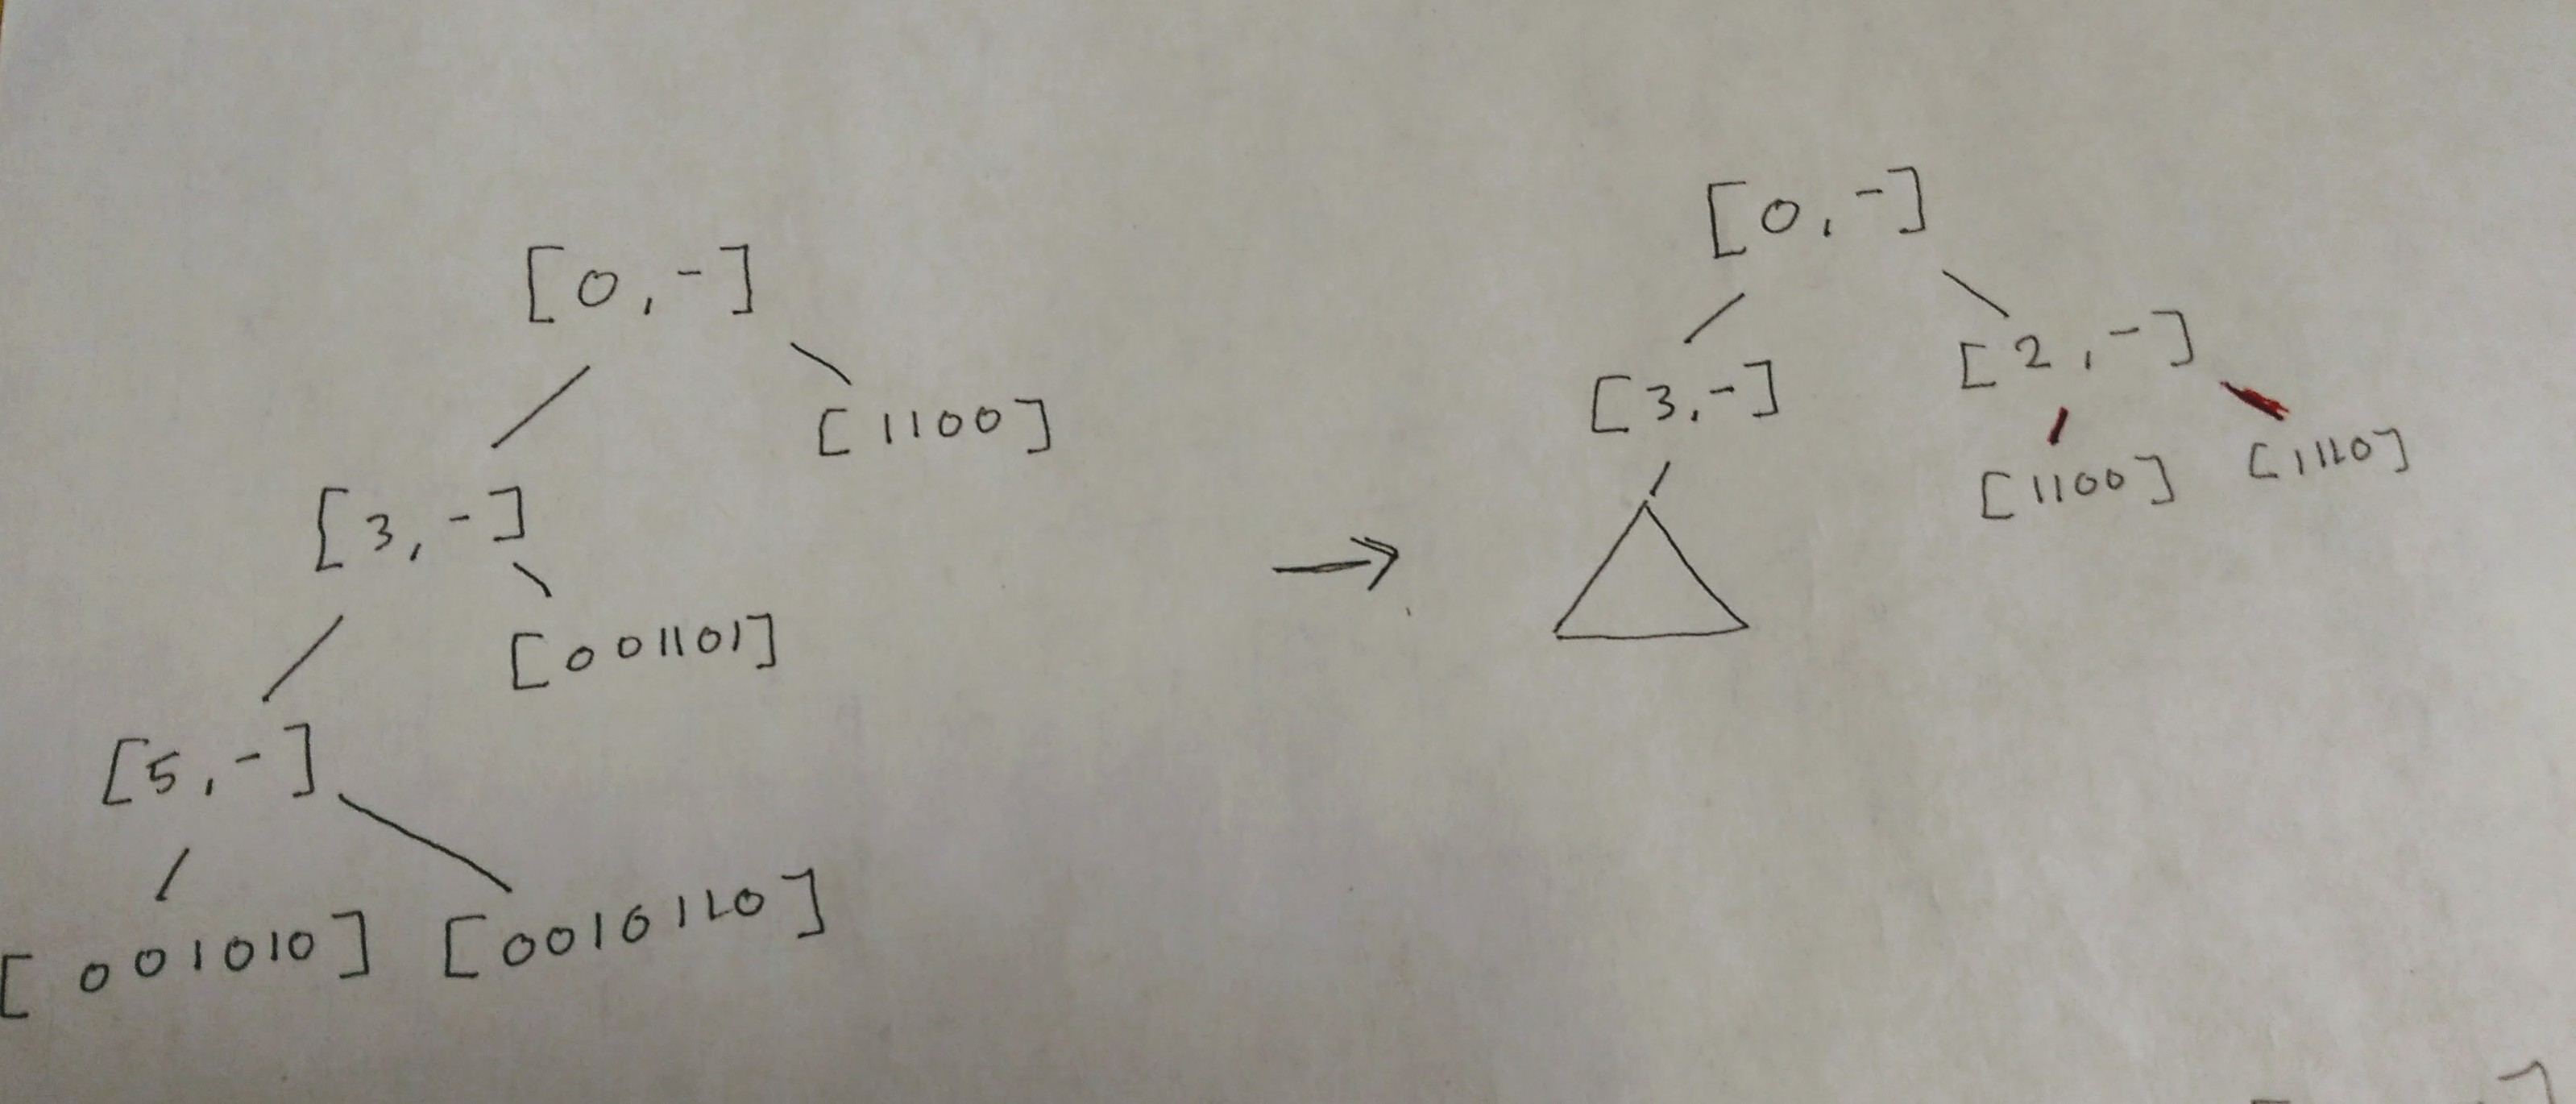
\includegraphics[scale=0.1]{trieEx1.jpg}
\end{center}
\caption{A visual example for example 12.2.2}
\end{figure}
\begin{ex}
Insert 001000 into an existing trie.
\end{ex}
\begin{itemize}
\item Search for 001000. Arrive at 001010.
\item The first index where 001000 and 001010 differ is at index 4. So we create a new node at index 4.
\end{itemize}
\begin{figure}[ht]
\begin{center}
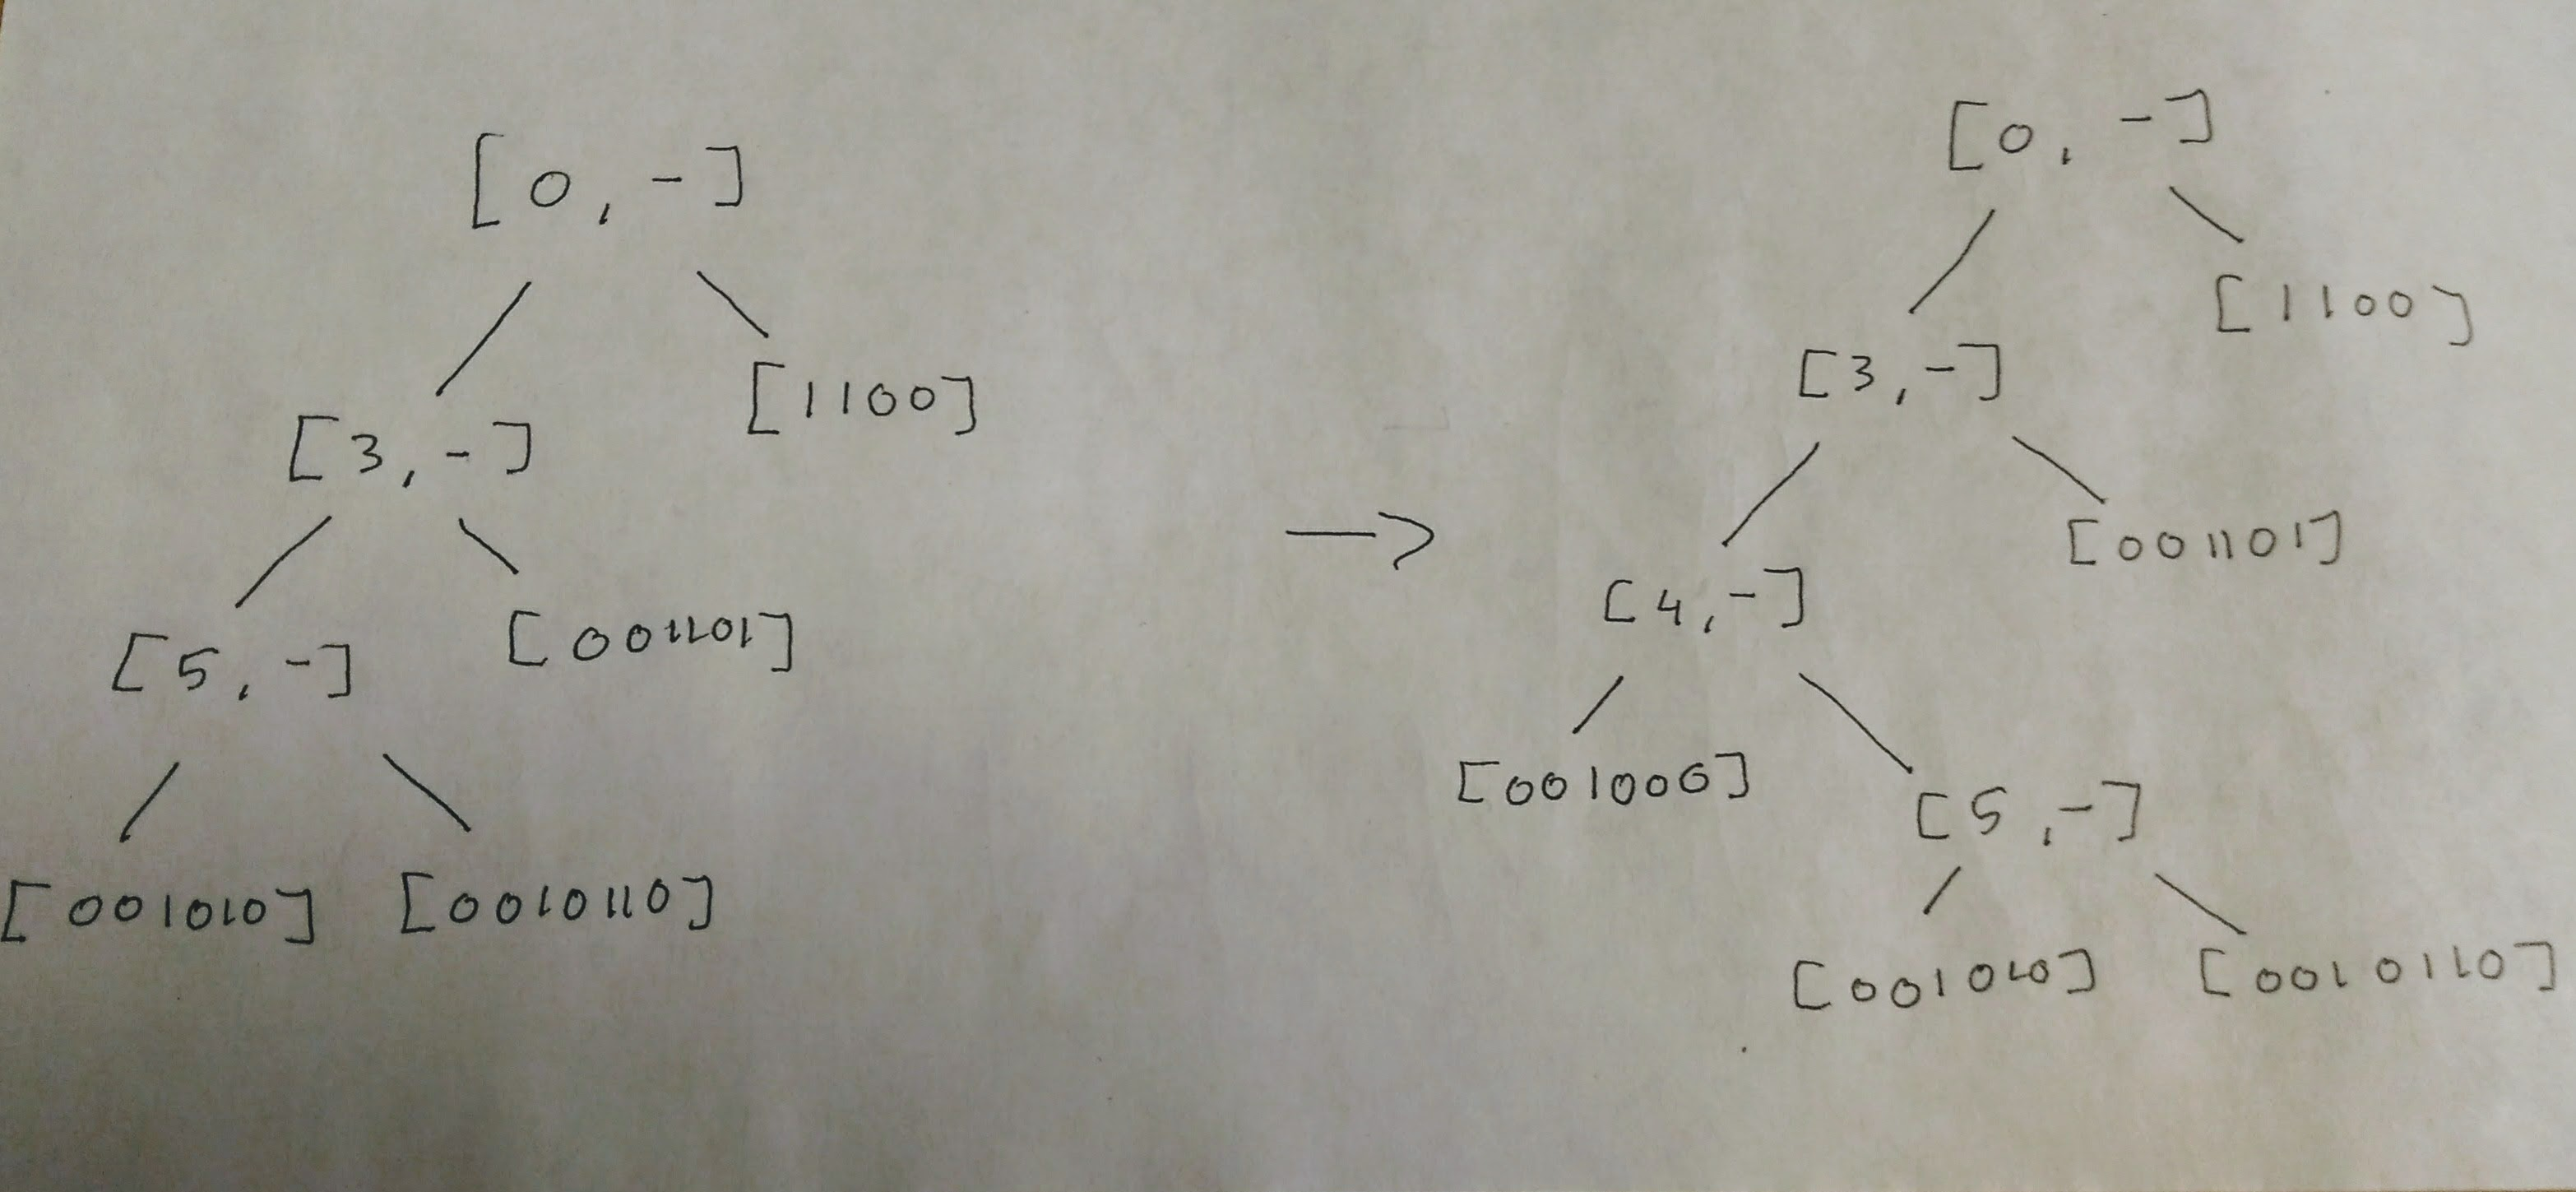
\includegraphics[scale=0.1]{trieEx2.jpg}
\end{center}
\caption{A visual example for example 12.2.3}
\end{figure}\newpage
\section{Multiway Tries}
Tries don't just have to represent binary strings. We can use \textbf{multiway tries} to represents any fixed alphabet $\Sigma$. In a trie, any node will have at most $|\Sigma|$ children. Of course, we can also implement a compressed multiway trie.
\begin{ex}
A compressed multiway trie (on the next page)
\end{ex}
\begin{figure}[ht]
\begin{center}
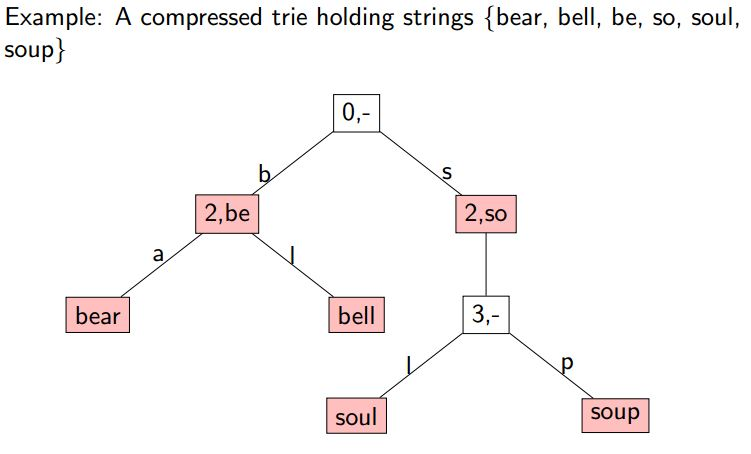
\includegraphics[scale=0.7]{mtrie2.jpg}
\end{center}
\caption{Courtesy of the CS 240 lecture slides. (I couldn't format this properly, so I'll just leave this here)}
\end{figure}
%END%
\end{document}